\subsubsection{Builder}

Il pattern \strong{Builder} serve per separare la costruzione di un oggetto
complesso dalla sua rappresentazione, in modo che lo stesso processo di
costruzione possa creare diverse rappresentazioni.

Il pattern può essere applicato quando:

\begin{itemize}
    \item l'algoritmo di creazione di un oggetto complesso dovrebbe essere
    indipendente dalle parti che compongono tale oggetto e come esse vengono
    assemblate;
    \item il processo di creazione deve permettere diverse rappresentazioni
    dell'oggetto che viene creato.
\end{itemize}

\begin{figure}[h!]
  \centering
  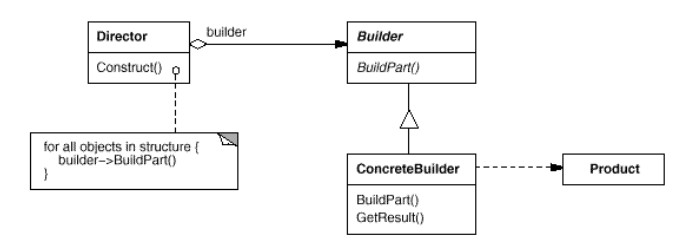
\includegraphics[scale=0.55]{imgs/builder.jpg}
  \caption{Diagramma delle classi del pattern Builder}
\end{figure}

All'utilizzo di un pattern Builder prendono parte diverse entità: un client, un
director, un builder astratto, un builder concreto e un product, risultato del
processo di creazione.

Il Client crea un oggetto Director e lo configura con il builder concreto
desiderato. Il Director utilizza tale builder, dietro interfaccia astratta, per
costruire il prodotto, che viene restituito dall'oggetto builder concreto al
Client.

\begin{figure}[h!]
  \centering
  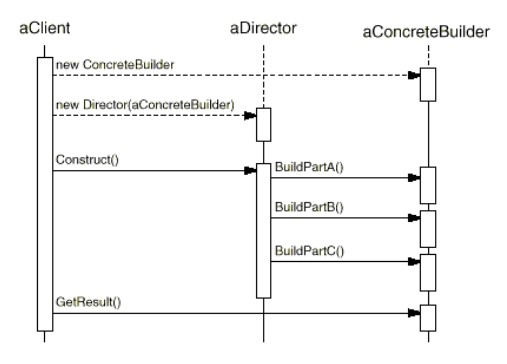
\includegraphics[scale=0.55]{imgs/builder_sd.jpg}
  \caption{Diagramma delle di sequenza del pattern Builder}
\end{figure}

\paragraph{Vantaggi}
\label{par:vantaggi}

\begin{itemize}
    \item L'interfaccia del Builder parmette di nascondere la rappresentazione e
    la struttura interna del prodotto, e come esso viene costruito.
    Per modificare la struttura interna del prodotto, e sufficiente
    aggiungere un builder.
    \item Isola il codice di rappresentazione e costruzione dei prodotti. Gli
    stessi ConcreteBuilder possono essere utilizzati da più Director.
    \item Il Builder costruisce il prodotto step-by-step, permettendo un
    controllo più fine sul processo di costruzione.
\end{itemize}

\paragraph{Considerazioni implementative}
\label{par:considerazioni_implementative}

\begin{itemize}
    \item Gli step del processo di costruzione sono definiti dall'interfaccia
    astratta del builder, pertanto tale interfaccia deve essere sufficientemente
    generale da permettere la costruzione di qualsiasi tipologia di prodotto.
    \item Non è necessario prevedere una superclasse astratta comune per il
    prodotto: i prodotti spesso differiscono pesantemente tra loro; inoltre, il
    client solitamente configura il director con una specifica classe builder
    concreta, pertanto è a conoscenza del prodotto concreto che viene creato.
\end{itemize}
